\chapter{Assays: Bone Marrow Mesenchymal Stem Cell Adhesion to ECM Produced by Cardiac Fibroblasts: An \emph{In Vitro} Model for Developing Cell-Based Therapies for the Heart}\label{Chap:Cardiac}

\section{Preface}
This chapter is done in equal partnership with Eric Schmuck working in the laboratory of Prof. Kurt W. Saupe. My primary role in this work was the implementation of the oscillatory flow device and readout whereas Eric was the driving force behind the \invitro\ model. Data acquisition and the design of experiments were a joint effort. The data presented here represents unfinished work that is expected to continue via further collaboration between the Beebe lab and the Saupe lab. For this reason, the goal of this chapter is to present preliminary data that shows potential for ways to study how cell-based therapies interact with the ECM of the heart.

\section{Introduction}
Heart disease is the leading cause of death in the United States with estimated costs of more than \$300 billion in 2010 \cite{Heron:2009kx,Lloyd-Jones:2010vn}. A major challenge in the area of heart disease stems from the poor regenerative capability of the heart. For this reason, stem-cells are being investigated for their potential to aid the regeneration of functional myocardium. Currently, conflicting data exists as to the efficacy or potential of stem-cell based therapies for treating heart disease with the best results showing modest improvement and the worst showing no improvement \cite{Assmus:2010qf,Beitnes:2009vn,Erbs:2007ve,Meyer:2006ly,Meyer:2009zr,Schachinger:2006bh,Wollert:2004ys}.

One of the primary challenges of implementing these therapies is the low retention rate of therapeutic cells in site of the treatment (typically $<$ 1-10\%) \cite{Freyman:2006nx,Ly:2009cr,Menasche:2010dq,Terrovitis:2009oq,Hofmann:2005tw}. The heart is highly vascularized and rhythmically contracts at approximately 60 beats per minute at rest, a rate that can as much as triple under sympathetic stimulation. This provides a difficult environment in which to promote attachment and adhesion. There is also much to learn in terms of when and where the therapeutic cells should be introduced and may vary from disease-to-disease, injury-to-injury, or even patient-to-patient.

Myocardial infarction (MI), cell death resulting from prolonged ischaemia, is one type of cardiac injury where stem-cell therapies may hold potential. The most common cause of the prolonged ischaemia is coronary artery disease (CAD). The extent of myocardial cell death varies with the length of ischaemia, collateral circulation, continuity of the blockage, and local demand for oxygen and nutrients \cite{Thygesen:2007ys,Alpert:2000ly}. After the infarct, there are 3-4 distinct phases of cardiac healing.

\begin{outline}
\1 Phase 1: Myocyte cell death (0-48 hours)
\2 Apoptosis is typically responsible for early cell death (6-8 hours) with necrosis occurring 12 hrs to 4 days after the infarct.
\1 Phase 2: Acute Inflammation (6 - 48 hrs)
\2 This phase is categorized by activation of the complement system and release of cytokines (IL-6, IL-8).  Within 6 hrs of the infarct, neutrophils migrate to the area to remove dead myocytes with numbers peaking between 24-48 post MI.  Lymphocytes, plasma cells, and macrophages also migrate to the area to remove dead myocytes. Inflammatory cells can persist in the tissue for several weeks leading to chronic inflammation as well, and is sometimes listed as a distinct healing phase.
\1 Phase 3: Granulation tissue (3 days - 4 wks post MI)
\2 Granulation is characterized by the deposition of new extracellular matrix proteins, first into the border zone between infarcted and non-infarcted tissue and later in the central area of the infarct.  The tissue becomes dense with myofibroblasts and inflammatory cells and is highly vascularized.
\1 Phase 4: Remodeling and Repair (3 wks - 1yr)
\2 This phase is characterized by accelerated ECM turnover and increased deposition in response to variation in wall stress.  Unique to heart healing is the persistence of fibroblasts in the scar area for long periods of time.  Fibroblasts have been found in the scar 17 years after the infarct \cite{Willems:1994fk}. In other tissues it is more common for fibroblasts to undergo apoptosis largely leaving the scar devoid of cells.
\end{outline}

Given our current knowledge of the events that occur post-infarction, there is an opportunity to develop \invitro\ models of these various stages of healing to help guide the development of new ways to improve current therapeutic methods. The heart has many unique biological and mechanical characteristics that make it difficult to model. Towards this end, we present a biomimetic approach for recapitulating many of the important microenvironmental characteristics of an infarct at various stages of healing. This approach is coupled with a recently developed microfluidic oscillatory flow adhesion assay that simulates the pulsatile environment of the infarct. An important characteristic of this particular adhesion assay is that a single data point can be acquired using hundreds of cells, enabling the use and study of rare cell populations, such as stem-cells, within these unique microenvironments. 

As illustrated in the phases of post-infarction healing, the microenvironment is dynamic, consisting of various ratios of different cell types and ECM at different times while the beating of the heart provides significant mechanical stresses. The system presented here consists of three main biological components: primary rat bone-marrow mesenchymal stem-cells (BMSCs), primary rat cardiac fibroblasts (CFs), and the ECM produced by the CFs. Many characteristics of the infarct microenvironment cannot be modeled using these three components. However, in this study, the focus is on the initial attachment of BMSCs to the site of an infarct. Modeling of the subsequent growth and proliferation is left for future work. Thus, our primary focus is to model different surfaces that might be presented to therapeutic cells upon delivery. To do this, various treatments are performed on these three components, in different combinations, to mimic different phases of post-infarction healing with respect to attachment. Attachment of the BMSCs in each of these environments is then tested using the oscillatory flow system to provide insight into potential avenues for improving delivery and retention of stem-cell therapies to the heart. Antibody-tethering is then used to improve BMSC attachment in order to demonstrate one potential avenue of improving this type of cell-based therapy.

\section{Results}

\subsection{Modeling Different Phases of Healing}
Cardiac fibroblasts play a large role in remodeling the heart post infarction and were thus chosen as a central component of the model. The fibroblasts and ECM produced by those fibroblasts are unique to each tissue \cite{Chang:2002ij,Fries:1994tg,Lekic:1997hc,Souders:2009kl,Chang:2002ij}. Thus, the goal in utilizing primary cardiac fibroblasts is to mimic the ECM of the heart as closely as possible, including the variety of ECM components and bound soluble factors that can play a role in adhesion, recruitment, and proliferation (\eg, VEGF, VWF, EGF, TGFb, FGF, ILGF, and HGFs) \cite{Franitza:2000fu,Hynes:2009bs,Iyer:2008fv,Vaday:2000kl,Vaday:2000dz}. Notably though, the ECM contains varying amounts of cells and cell debris at different stages in the healing process, a characteristic which can be modeled in some ways via cell lysis. Decellularization via cell lysis can be used to remove the CFs while leaving behind the deposited ECM. Different protocols can be used to produce ECM with various amounts of remaining cell debris. This tunability is leveraged here to produce three distinct conditions. The first is an unperturbed matrix that still contains the CFs. This scenario is closest to the late end of Phase 3 and Phase 4 where the scar from the infarct consists largely of fibroblasts and ECM. The second condition is an ECM that is without CFs and nearly devoid of cell debris, a situation that mimics the ECM at the end of Phase 2, the phase in which immune cells remove cell debris. The third condition is produced using a lysis method that leaves a significant amount of cell debris to mimic the ECM of an infarct shortly after myocyte death (Phase 1). It is likely that initial attachment of therapeutic cells will depend significantly upon the presence of cell debris, availability and presentation of the ECM and potential interaction with supporting fibroblasts. The use of an adhesion assay will allow us to functionally test the relative importance of these interactions and provide insight into ways to facilitate attachment and begin addressing a significant hurdle to stem-cell therapies for the heart. Characterization of the three different conditions\slash models is presented based on the progression of the healing process.

\begin{outline}
\1 Model 1: Post Myocyte Death
\1 Model 2: Post Removal of Cell Debris
\1 Model 3: Scar Formation and Late-Stage Healing
\end{outline}

\paragraph{\textbf{Note}:} It will still be necessary to learn more about the specific differences of the ECMs produced by the different lysis methods. For example, it is expected that AH without Triton will produce results similar to PAA. If this is true, this will provide a more controlled and specific difference between Model 1 and 2 for future characterization.

\subsection{Model 1: Post Myocyte Death}
Peracetic acid (CH$_{3}$CO$_{3}$H or PAA) can be used to decellularize the CF ECM but leaves behind a significant amount of CF cell debris. The debris left behind using PAA may help to mimic an ECM surface shortly after cell death as these components may interact or interfere with the attachment of therapeutic cells. The level of debris can be seen more clearly when compared to ECM that has been decellularized using a mixture of ammonium hydroxide and Triton (subsequent references to the NH$_{4}$OH\slash Triton mixture and method are abbreviated as AH). Despite differences in the staining protocol, morphological differences can be seen in Fig \ref{Chap:Cardiac:fig:ecmEosin} that suggest more cell material is left behind in the case of PAA. In the case of AH, the ECM fibers can be more easily discerned. 

\begin{figure}[!ht]
\centering
\begin{tabular}{ll}
A) PAA & B) AH \cr
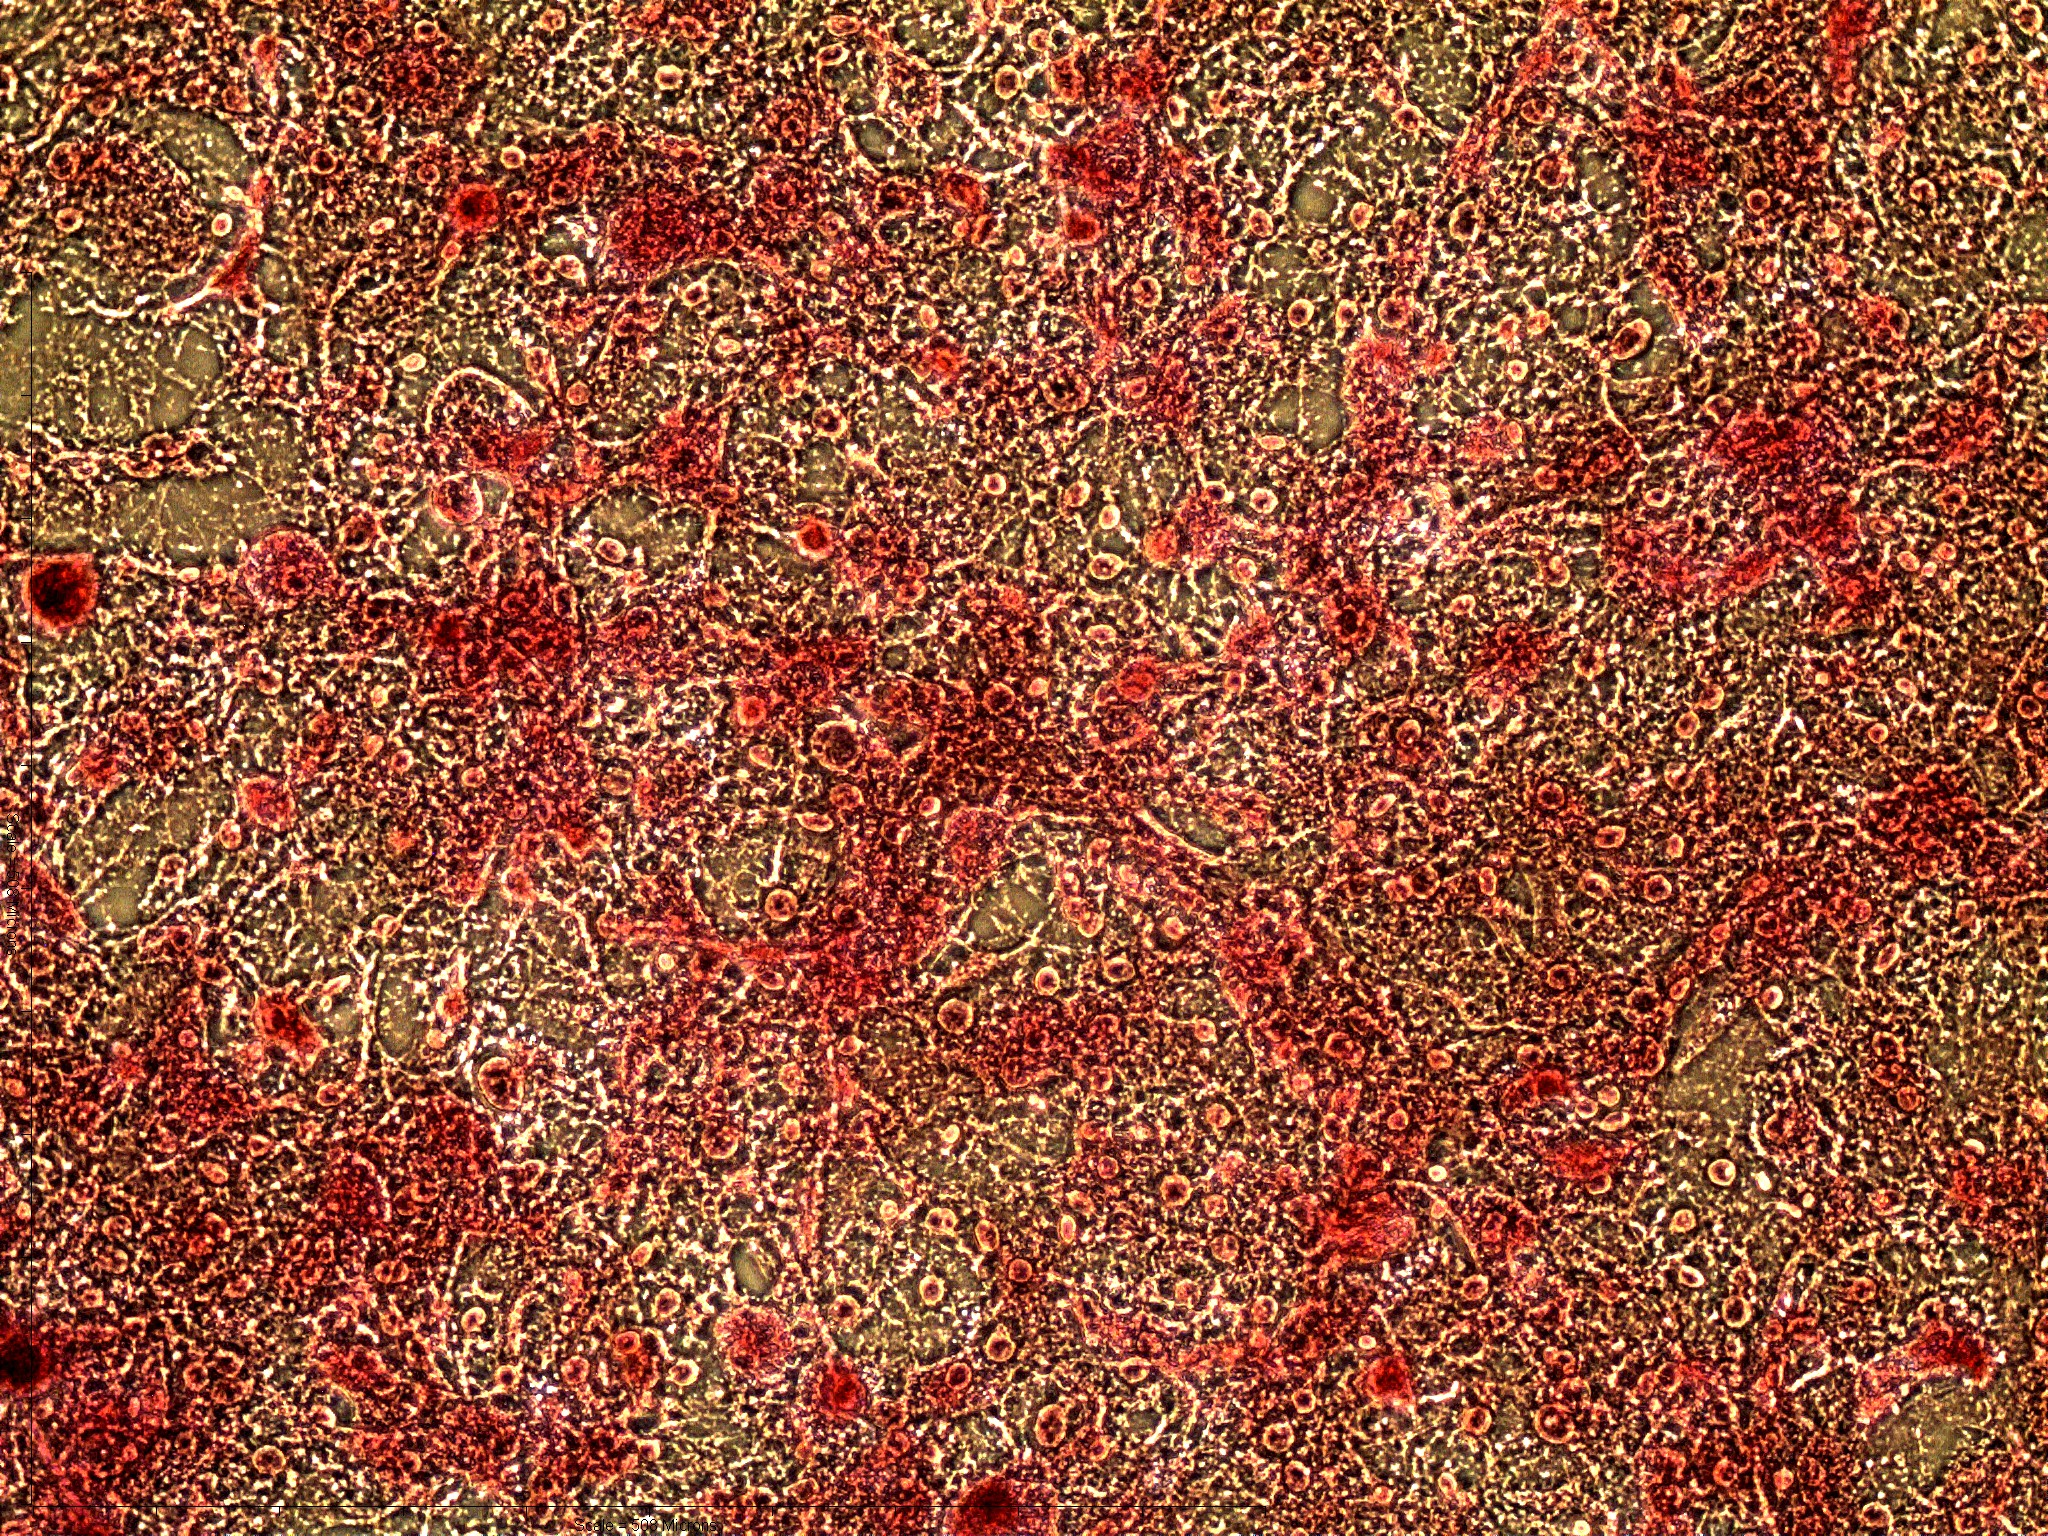
\includegraphics[width=3in]{PAA20X.jpg} & 
\includegraphics[width=3in]{AH20X.pdf} \cr
\end{tabular}
\caption{\textbf{Histology staining of CF-produced ECM}. A) ECM produced by CFs in microchannels, prepared using PAA, and stained using hematoxylin and eosin. B) ECM produced by CFs in microchannels, prepared using AH, and stained using only eosin. The scale bar in B applies to both images.}
\label{Chap:Cardiac:fig:ecmEosin}
\end{figure}

Preliminary staining and mass spectrometry data suggest fibronectin as the primary component of the matrix followed by Collagen 1, 3 and other various fibular and basement collagens and elastin (Appendix \ref{App:Cardiac}).

Further characterization of this ECM is to be completed by Eric Schmuck.

\subsection{Model 2: Post Removal of Cell Debris}
AH is more effective at removing cell debris than PAA and produces an ECM that may be more appropriate for modeling the ECM at an the site of an infarct after cell debris has been removed by the immune system. Fig \ref{Chap:Cardiac:fig:ecmImmunostain} shows immunostaining results for ECM cultured and decellularized for different lengths of time. Fig \ref{Chap:Cardiac:fig:ecmImmunostain}A shows ECM after 2 hrs of AH treatment and illustrates the layered nature of the ECM, green showing fibronectin and red showing collagen I. Blue, which is indicative of nuclear material remaining after AH, is only present at low levels. Fig \ref{Chap:Cardiac:fig:ecmImmunostain}B illustrates that increased ECM thickness results in more cellular material being left behind after the same AH treatment, as indicated by the diffuse blue color. If AH treatment is kept short, more nuclear material can be seen and is less diffuse. These images illustrate the ability to alter the AH protocol to leave various amounts of cell debris after treatment.

\begin{figure}[!ht]
\centering
\begin{tabular}{lll}
A) Thin ECM & B) Thick ECM & C) Short AH Treatment\cr
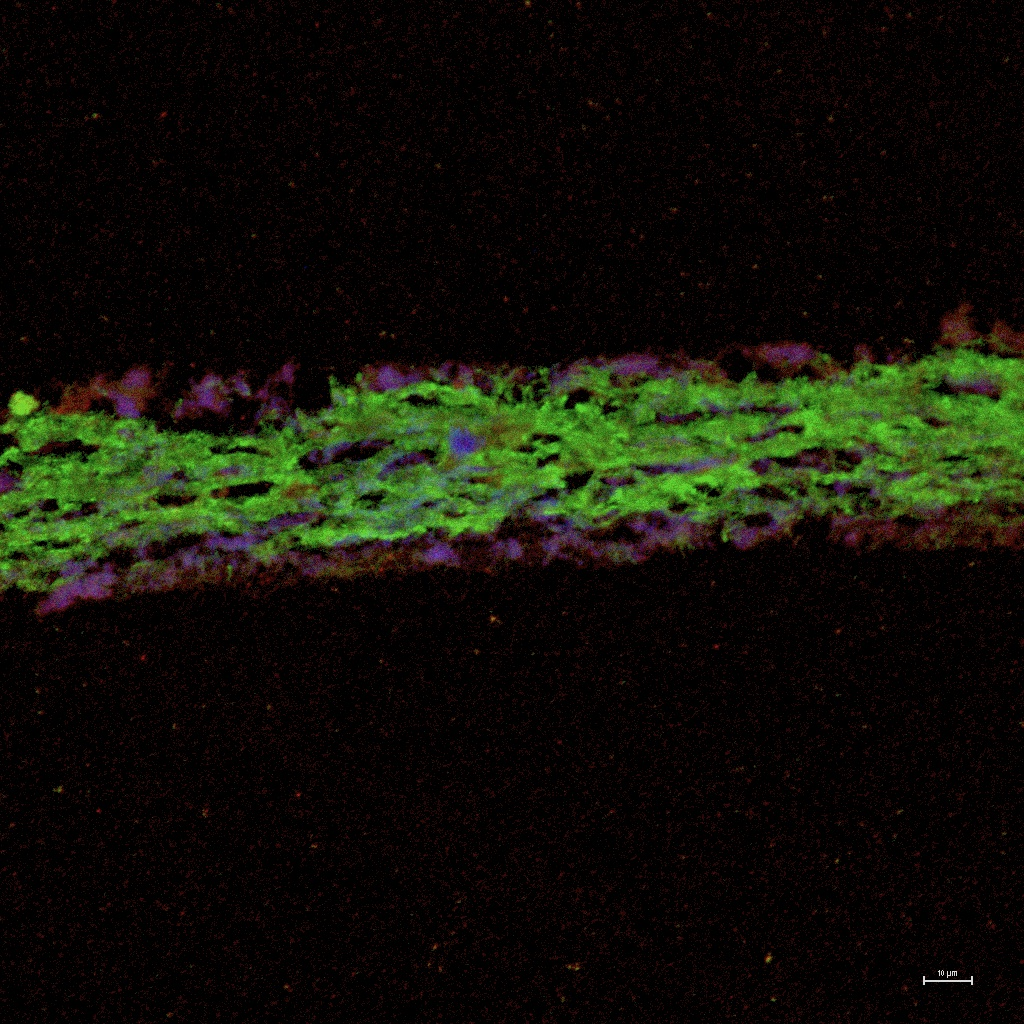
\includegraphics[width=1.8in]{StainThin.jpg} & 
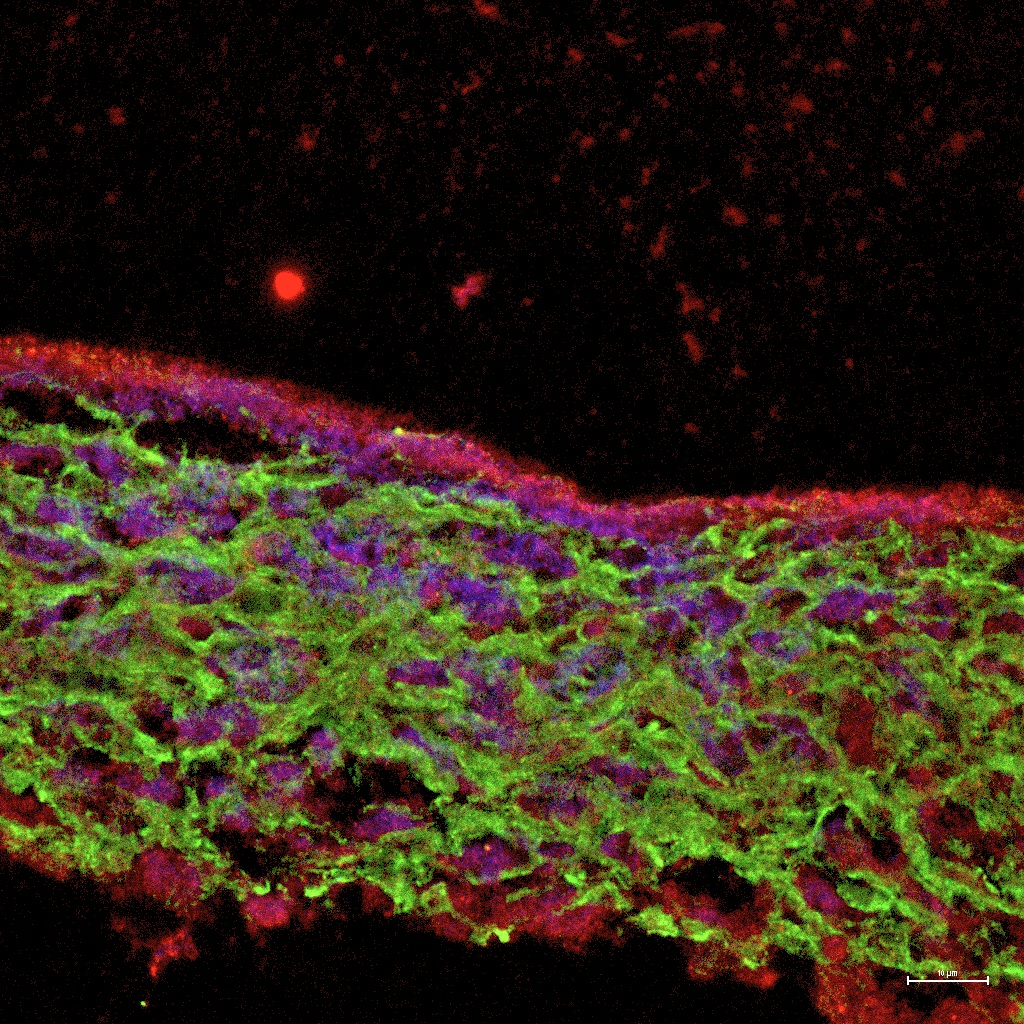
\includegraphics[width=1.8in]{StainThick.jpg} &
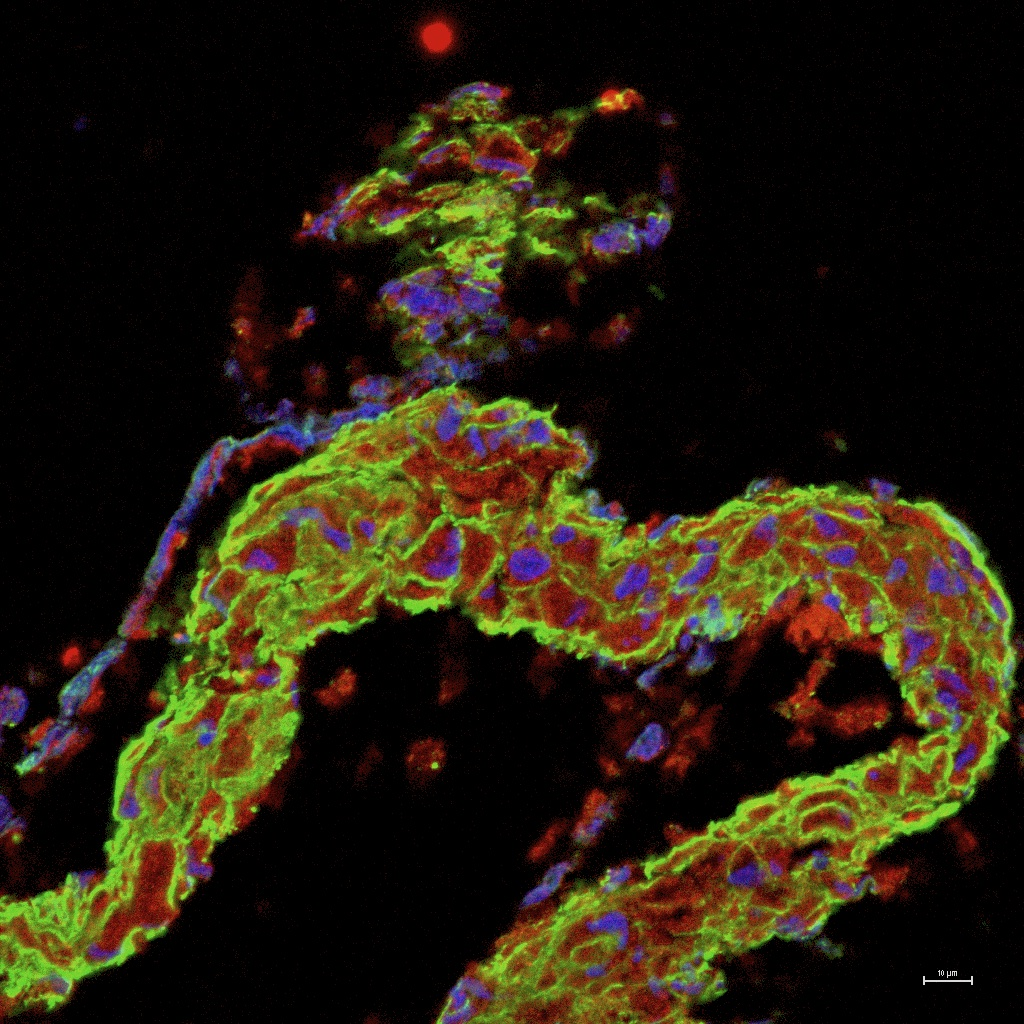
\includegraphics[width=1.8in]{StainShort.jpg} \cr
\end{tabular}
\caption{\textbf{Immunostaining of CF ECM prepared using AH}.  The ECM in the images was produced by CFs cultured in flasks, embedded in paraffin and sectioned to 5 \textmu m thick providing a cross-section view of the ECM. Blue = DAPI, Red = Collagen I, Green = Fibronectin. Scale bars are 10 \textmu m. A) Example of ``thin'' ECM exposed for 2 hrs to AH. B) Example of ``thick'' ECM exposed for 2 hrs to AH. C) Example of thin ECM exposed for $<$ 10 min of AH.}
\label{Chap:Cardiac:fig:ecmImmunostain}
\end{figure}

Further characterization of this ECM is to be completed by Eric Schmuck.

\subsection{Model 3: Scar Formation and Late-Stage Healing}
CF cells embedded in their own self-produced ECM recapitulate aspects of scars typical of late-stage healing where the injury site is primarily comprised of fibroblasts and connective tissue.

Additional characterization of how CFs remaining in the matrix can potentially interact with attachment of therapeutic cells is also expected be part of future work.

\subsection{BMSC Adhesion}
As described in Chapter \ref{Chap:TumorCellAdhesion}, a descending log frequency sweep is used to observe cell adhesion of a single population of cells over a range of shear-stresses. Characterizations performed in Chapter \ref{Chap:Oscillator} show that shear-stress is linearly related to the frequency of oscillation given that amplitude of the oscillation remains constant. The descending sweep provides an opportunity to observe and quantify the initial BMSC attachment event to the CF ECM that is thought to be a critical challenge of similar strategies for treating MI. By using oscillatory flow, small numbers of cells can be used to study this interaction and is an important consideration when working with stem-cells.

Adhesion results are interpreted using a log-normal cumulative distribution function (LNcdf). The parameters and interpretation of this distribution are discussed in Chapter \ref{Chap:TumorCellAdhesion}. The two parameters that are measured from each set of adhesion data are the median shear-stress, $\tau_{50}$, and $\sigma$, a measure of the spread or heterogeneity in the data on the log scale.

\subsubsection{Model 1 \vs\ Model 2: Influence of Cell Debris}
Fig \ref{Chap:Cardiac:fig:1v2} compares BMSC adhesion in Model 1 and 2. In this case a very dramatic result is observed. Data suggests that ECM prepared using AH results in a $\tau_{50}$ for BMSC adhesion that is nearly a full order of magnitude higher than with the ECM prepared using PAA. Results of fitting the data with a LNcdf are summarized beside the plot.
\begin{figure}[!t]
\centering
\imagetop{\includegraphics[width=3.5in]{Lysis.pdf}}
\imagetop{\begin{tabular}{cr@{.}lcc}
\multicolumn{5}{c}{LNcdf Fits}\cr\toprule
Lysis & \multicolumn{2}{c}{$\tau_{50}$ [Pa]} & Sigma & R$^{2}$\cr\midrule
NH$_{4}$OH & 0&047 & 0.67 & 0.99\cr
NH$_{4}$OH & 0&040 & 0.87 & 0.98\cr
NH$_{4}$OH & 0&052 & 0.78 & 0.97\cr
PAA & 0&0067 & 1.40 & 0.99\cr
PAA & 0&0064 & 1.80 & 0.98\cr\bottomrule
\end{tabular}}
\caption{\textbf{BMSC adhesion to decellularized ECM}. (blue) Model 1. ECM was prepared using PAA. (red) Model 2. ECM was prepared using NH$_{4}$OH (AH). (table) $\tau_{50}$ and $\sigma$ are the median shear stress and sigma determined from the curve fit of the data. `Control' is used to indicate that these cells were not labeled with the tagging antibody used in later experiments.}
\label{Chap:Cardiac:fig:1v2}
\end{figure}

%\begin{table}[!ht]
%\caption{\textbf{Log-normal fitting results}.}
%\centering
%\label{Chap:Cardiac:tab:1v2}
%\end{table}


\subsubsection{Model 2 \vs\ Model 3: Influence of CFs}

Preliminary adhesion data has not been acquired yet for this condition and will be the focus of continued collaboration between the laboratories of Prof. Beebe and Prof. Saupe.

\subsection{Increased Attachment via Antibody Tethering}
The use of antibodies to modify adhesion is well established. Most commonly, antibodies are used to block specific interactions in functional assays of adhesion \cite{GIAVAZZI:1993ty}. Antibodies are also used to promote adhesion to surfaces, typically in applications aimed at isolated rare cells from large volumes, either through the use of beads or microscale structures \cite{Nagrath:2007bs,Cristofanilli:2004hp}. In contrast, there are very few instances where an adhesion interaction is engineered between two biological (\ie, non-engineered) components such as two different primary cell types or a natural ECM and a primary cell type. In this case, BMSCs will be tethered to the ECM using antibodies to CD44, a BMSC surface marker, and fibronectin, the primary component of the CF ECM. The situation is similar to the binding of beads to a protein where, instead of the bead, the BMSC will be the object functionalized with the antibody. This is done by joining the two antibodies via biotin-streptavidin chemistry to create a hetero-bifunctional linker. The affinities of the antibodies to their ligands have been observed previously using immuno-histochemistry in the Saupe lab. 

The investigation serves as a proof of concept that physical linking of the therapeutic cells to the diseased site may be a viable approach for increasing retention and demonstrates the use of an adhesion assay and model of cardiac ECM to assess the efficacy of such methods. Given this scope, the potential effects of such a strategy on subsequent growth and differentiation of the BMSCs is left to future work and others interested in engineering the interaction of these cells with cardiac tissue. Some potential advantages of this approach are the wide availability of antibodies to stem-cell markers and other proteins, providing significant flexibility to address potential effects of the antibodies on stem-cell fate.

\begin{figure}[!t]
\centering
\begin{tabular}{p{0.3cm}c}
A) & \imagetop{\includegraphics[width=3.5in]{Tagging.pdf}}
\imagetop{\begin{tabular}{cr@{.}lcc}
\multicolumn{5}{c}{LNcdf Fits}\cr\toprule
Ab Tag & \multicolumn{2}{c}{$\tau_{50}$ [Pa]} & Sigma & R$^{2}$\cr\midrule
Y & 0&057 & 0.67 & 0.98\cr
Y & 0&084 & 0.44 & 0.95\cr
Y & 0&058 & 0.77 & 0.98\cr
N & 0&047 & 0.67 & 0.99\cr
N & 0&040 & 0.87 & 0.98\cr
N & 0&052 & 0.78 & 0.97\cr\bottomrule
\end{tabular}}\cr
B) & \imagetop{\includegraphics[width=3.5in]{Tagging2.pdf}}
\imagetop{\begin{tabular}{cr@{.}lcc}
\multicolumn{5}{c}{LNcdf Fits}\cr\toprule
Ab Tag & \multicolumn{2}{c}{$\tau_{50}$ [Pa]} & Sigma & R$^{2}$\cr\midrule
Y & 0&0068 & 1.40 & 0.98\cr
Y & 0&0072 & 1.60 & 0.98\cr
N & 0&0067 & 1.40 & 0.99\cr
N & 0&0064 & 1.80 & 0.98\cr\bottomrule
\end{tabular}}\cr
\end{tabular}
\caption{\textbf{BMSC adhesion to decellularized ECM}. A) Adhesion of antibody tagged BMSCs \vs\ control on AH prepared ECM. B) Adhesion of antibody tagged BMSC \vs\ control on PAA prepared ECM.}
\label{Chap:Cardiac:fig:tagging}
\end{figure}
Fig \ref{Chap:Cardiac:fig:tagging} shows initial effects of the antibody tagging method on BMSC adhesion to ECM prepared via both lysis methods. The five data points consistently estimated the antibody tagged BMSCs to be more adherent than the control BMSCs on the AH prepared ECM. There was no such ordering in the case of the PAA prepared ECM. This may indicate that cell debris is interfering with interaction between the BMSCs and the ECM which agrees with previous results. Also, the median shear-stress for the PAA prepared ECM was nearly an order of magnitude lower than the median for the AH prepared ECM for both the tagged and control case. The difference in adhesion observed here upon removal of cell debris is obviously larger than any potential effect that the antibody tagging provided. However, given the log-scale of the plots, the potential effect of the antibody tagging should not be ignored as the absolute change in the median shear stress may be significant. 

\section{Additional Adhesion Comparisons}
The adhesion of BMSCs with and without antibody tags were tested on tissue culture plastic (TCP) and TCP treated for 30 min with 100 \textmu g/mL of fibronectin. These tests were included as a means for others to gauge the levels of adhesion relative to more well known substrates. Fig \ref{Chap:Cardiac:fig:standards} summarizes these results. It appears that the addition of fibronectin did have an effect on BMSC adhesion. Instead of changing the $\tau_{50}$, the addition of fibronectin reduced the value of sigma, indicating an increased role in a specific mechanism of adhesion (Chapter \ref{Chap:TumorCellAdhesion}). This would be expected as TCP does not offer any specific means of adhesion other than via non-specific charge-based interactions. CD44, which is expressed on the surface of BMSCs is known to interact with fibronectin naturally and may be one way in which the interaction of the BMSCs was made more specific.

\begin{figure}[!t]
\centering
\imagetop{\includegraphics[width=3.5in]{Substrate.pdf}}
\imagetop{\begin{tabular}{cr@{.}lcc}
\multicolumn{5}{c}{LNcdf Fits}\cr\toprule
Substrate & \multicolumn{2}{c}{$\tau_{50}$ [Pa]} & Sigma & R$^{2}$\cr\midrule
TCP+,+ & 0&012 & 1.05 & 0.99\cr
TCP+,- & 0&014 & 1.19 & 0.99\cr
TCP-,+ & 0&013 & 1.78 & 0.97\cr
TCP-,- & 0&011 & 1.62 & 0.98\cr\bottomrule
\end{tabular}}
\caption{\textbf{BMSC adhesion to common substrates}. The first $\pm$ sign indicates the whether the TCP was treated with 100 \textmu g/mL of fibronectin or not while the second indicates whether the BMSCs were tagged with antibody to fibronectin.}
\label{Chap:Cardiac:fig:standards}
\end{figure}

\section{Discussion and Conclusion}
Overall, preliminary results suggest BMSC adhesion is highly dependent on the presence of cell debris. Further characterization of the ECMs produced by each protocol as well as additional repeats of the adhesion experiments are necessary to make more substantial conclusions concerning the potential implications for improving retention of cell-based therapies. Additional data is also needed to better illustrate the potential for molecular tethering strategies to improve therapeutic cell retention. However, initial results suggest that tethering strategies are subject to the effects of cell debris. Instead, it may be that a greater increase in retention will be achieved by maximizing the exposure of the underlying ECM at the treatment site.

Next steps will be to explore the influence of Triton on adhesion by comparing lysis using NH$_{4}$OH with and without Triton. This could provide a more subtle, specific, and quantifiable difference between the lysis conditions that will aid future work. Also, the use of blocking antibodies to functionally test which ECM components are the primary mediators of adhesion will be useful in guiding future strategies for improving cell retention. Cell debris will also be added exogenously to the system as an addition test of the current hypothesis.

\section{Methods}

\subsection{PAA Lysis}
CFs are washed in 3-4 changes of water to initiate cell lysis by hypotonic shock.  The cells are then incubated in 0.15\%PAA for 24 - 48hrs, followed by 4 changes of water.  Finally, the ECM is equilibrated with serum free DMEM until the experiment is run.

\subsection{AH Lysis}
CFs are washed in 3-4 changes of water to initiate cell lysis by hypotonic shock.  The cells are then incubated in decellularizing solution containing 40mM NH4OH and 0.5\% Trition-X 100 for 24 - 48 hrs, followed by 4 changes of water.  Finally, the ECM is equilibrated with serum free DMEM until the experiment is run.

\subsection{CF Isolation and Culture}
CF isolation is based on previous work in the literature \cite{Baharvand:2005mi,Dubey:1997qa}. Male Lewis Rats (240-300g) are sacrificed by CO2 asphyxiation, hearts rapidly excised and atria removed and placed into ice cold PBS with 1\% penicillin/Streptomycin.  Hearts are finely minced then placed into 10mLs digestion media (DMEM, 73U/mL Collagenase 2, 12μg/mL Pancreatin (4x)) and incubated at 37°C with agitation for 35 minutes.  The digest mixture is centrifuged at 1000xg for 20 minutes at 4°C.  Resulting cell pellet is suspended in 10mLs of fresh digestion media and incubated at 37°C with agitation for 30 minutes.  The resulting digest is sieved through a 70μm cell strainer and digest solution diluted with 10mLs of Culture media (DMEM, 10\% FBS, 1\% Penicillin/Streptomycin).  The cell suspension is then centrifuged at 1000xg for 20 minutes at 4°C.  The cell pellet is suspended in 16mLs culture media and plated into 2 T75 culture flasks.  The cells are allowed to attach under standard culture conditions (37°C, 5\% CO2, 100\% humidity) for 2 hrs, then non-adherent cells removed by washing with PBS and culture media replaced. Primary CFB cultures are usually confluent in 4-7 days.

\subsection{BMSC Isolation and Culture}
BMSC isolation is based on previous work in the literature \cite{Baharvand:2005mi,Tropel:2004pi}. Male Lewis Rats (240-300g) are sacrificed by CO2 asphyxiation. Femurs and Tibias are bilaterally excised and soft tissue removed.  The bones are placed in ice cold PBS with 1\% penicillin/Streptomycin.  Ends of the bones are then removed and an 18 gauge needle and syringe used to flush the shafts of the bones with Culture media (DMEM, 10\% FBS, 1\% Penicillin/Streptomycin).  The resulting bone marrow is further dispersed by passage through a 21 gauge needle.  Cell suspension is then centrifuged at 1000xg for 10 minutes at 4°C and plated into a 100mm culture dish.  The cells are allowed to attach under standard culture conditions (37°C, 5\% CO2, 100\% humidity) for 24 hrs, then non-adherent cells removed by washing with PBS and culture media replaced.

\subsection{Adhesion Assay}
Please refer to Chapter \ref{Chap:Oscillator} and \ref{Chap:TumorCellAdhesion}.





